% !TEX root = ../../main.tex

\subsection{Impact of framework structure on transition mechanics}%
\label{dut:comparison}

While the discovery of the NGA transition in DUT-49 was a result 
of serendipity, it opens the door to a rational design approach 
to modify the extent and the location of the phenomenon. In principle,
there are several avenues that could be taken in order to tune the 
contraction mechanics.
\begin{itemize}
    \item Changing the range of metastability of the open pore state.
    \item Decreasing the porosity of the closed pore state.
    \item Increasing the capacity of the open pore form.
\end{itemize}
These factors are bound to be tightly interlinked, with a slight 
alteration in one possibly leading a shift in all. For example, the 
addition of a stabilizing group which would increase the tensile 
strength of the linker is also likely to decrease the porosity 
of the entire system.

There are a range of physicochemical modifications available to 
tune the properties of the framework, many already employed in the
MIL-53 and MIL-47 family of flexible MOFs.
Through functionalisation or modification of the linker, the strength of the guest-guest
and guest-host interactions is affected, as evidenced by the different
gate opening behaviour with nitrogen and water on several functionalised
versions on MIL-53~\cite{biswasNewFunctionalizedFlexible2011}.
In the case of DUT-49, moieties grafted to the central strut or changes
in the linker backbone are also likely to affect its buckling behaviour.
The use of a different metal as the node, has succeeded in changing the 
mechanical response of MIL-53~\cite{yotImpactMetalCentre2016}. This 
approach is likely have less impact on DUT-49, as the mechanism of 
contraction is due to linker flexibility.
A common rational design methodology is the so-called isoreticular design,
where topologically isomorphic MOFs are synthesised through progressive elongation
of the linker. Another path to controlling flexibility is manipulation of crystal 
size, as it has already been shown by \citet{krauseEffectCrystalliteSize2018}.
Finally, structural defects, of which a description was given 
in \autoref{def}, are another degree of freedom to consider for NGA 
tunability. Approaches such as mixed linkers synthesis and vacancy defects
may allow for fine-grain influence of framework stiffness.

\subsubsection{Behaviour of isoreticular materials}

Adsorption 

\autoref{dut:fgr:dut-reticular} shows the dataset recorded on the 
non-interpenetrated versions of the material.

\begin{figure}[htb]
    \centering
    \begin{subfigure}{0.33\linewidth}
        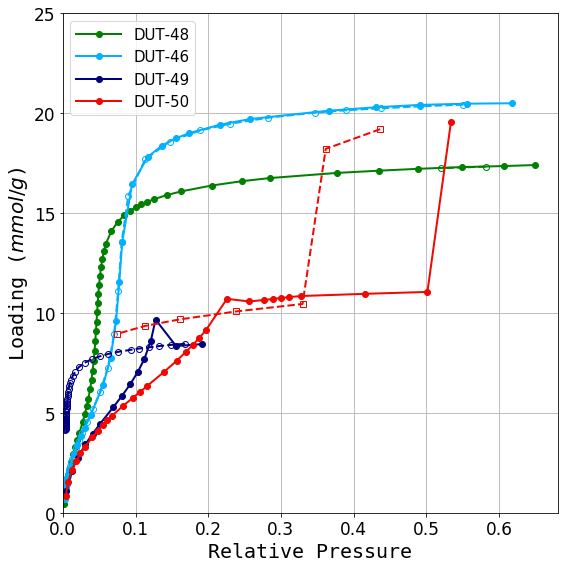
\includegraphics[width=\linewidth]{butane/dut-reticular-reg}%
        \caption{}\label{dut:fgr:dut-reticular-reg}
    \end{subfigure}%
    \begin{subfigure}{0.33\linewidth}
        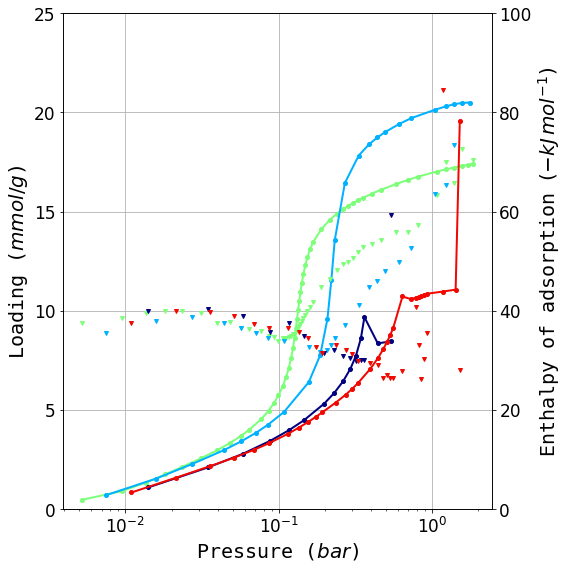
\includegraphics[width=\linewidth]{butane/dut-reticular-log}%
        \caption{}\label{dut:fgr:dut-reticular-log}
    \end{subfigure}%
    \begin{subfigure}{0.33\linewidth}
        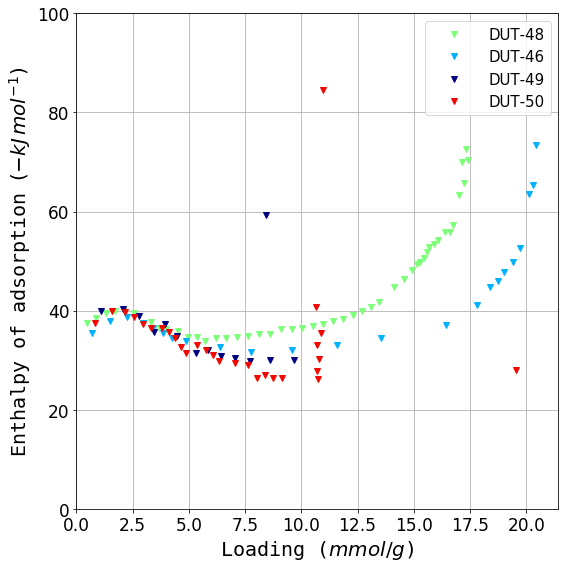
\includegraphics[width=\linewidth]{butane/dut-reticular-enth}%
        \caption{}\label{dut:fgr:dut-reticular-enth}
    \end{subfigure}%
    \caption{(a) Experimental adsorption isotherms for DUT-48, DUT-46, DUT-49 and 
    DUT-50. Enthalpy points are omitted for clarity. (b) A logarithmic plot of 
    isotherms and enthalpy curves, to highlight the low pressure region. 
    (c) Enthalpy as a function of loading for these materials.}%
    \label{dut:fgr:dut-reticular}
\end{figure}


The isotherms in \autoref{dut:fgr:dut-reticular-reg} show that only DUT-49 
and DUT-50 undergo NGA, one around \(0.15~p/p_0\) and the other at a higher 
relative pressure around \(0.25~p/p_0\).

Indeed, the results follow a predictable trend. With an increase of linker 
size, a higher overall capacity is available from the 

In DUT-50, the structure is seen to re-open around \(0.5~p/p_0\), although 
the pressure is not high enough to obtain a fully \textbf{op} form.
The transition to the \textbf{cp} phase is 

\autoref{dut:fgr:dut-reticular-interp} presents isotherms and enthalpy on 
DUT-151 and DUT-152, both interpenetrated nets.

\begin{figure}[htb]
    \centering
    \begin{subfigure}{0.5\linewidth}
        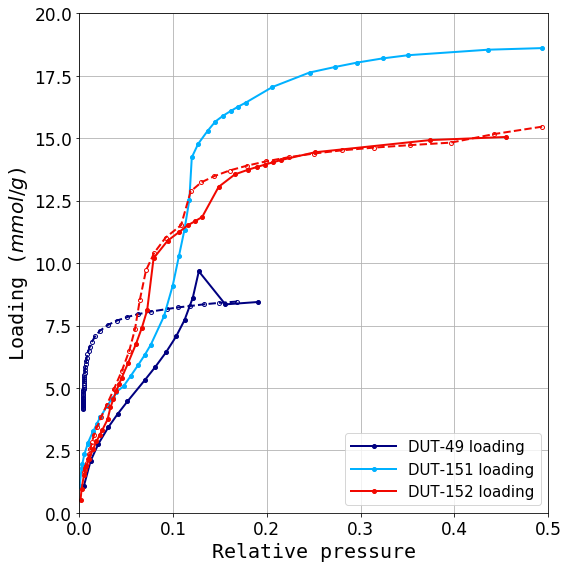
\includegraphics[width=\linewidth]{butane/dut-reticular-interp-reg}%
        \caption{}\label{dut:fgr:dut-reticular-interp-reg}
    \end{subfigure}%
    \begin{subfigure}{0.5\linewidth}
        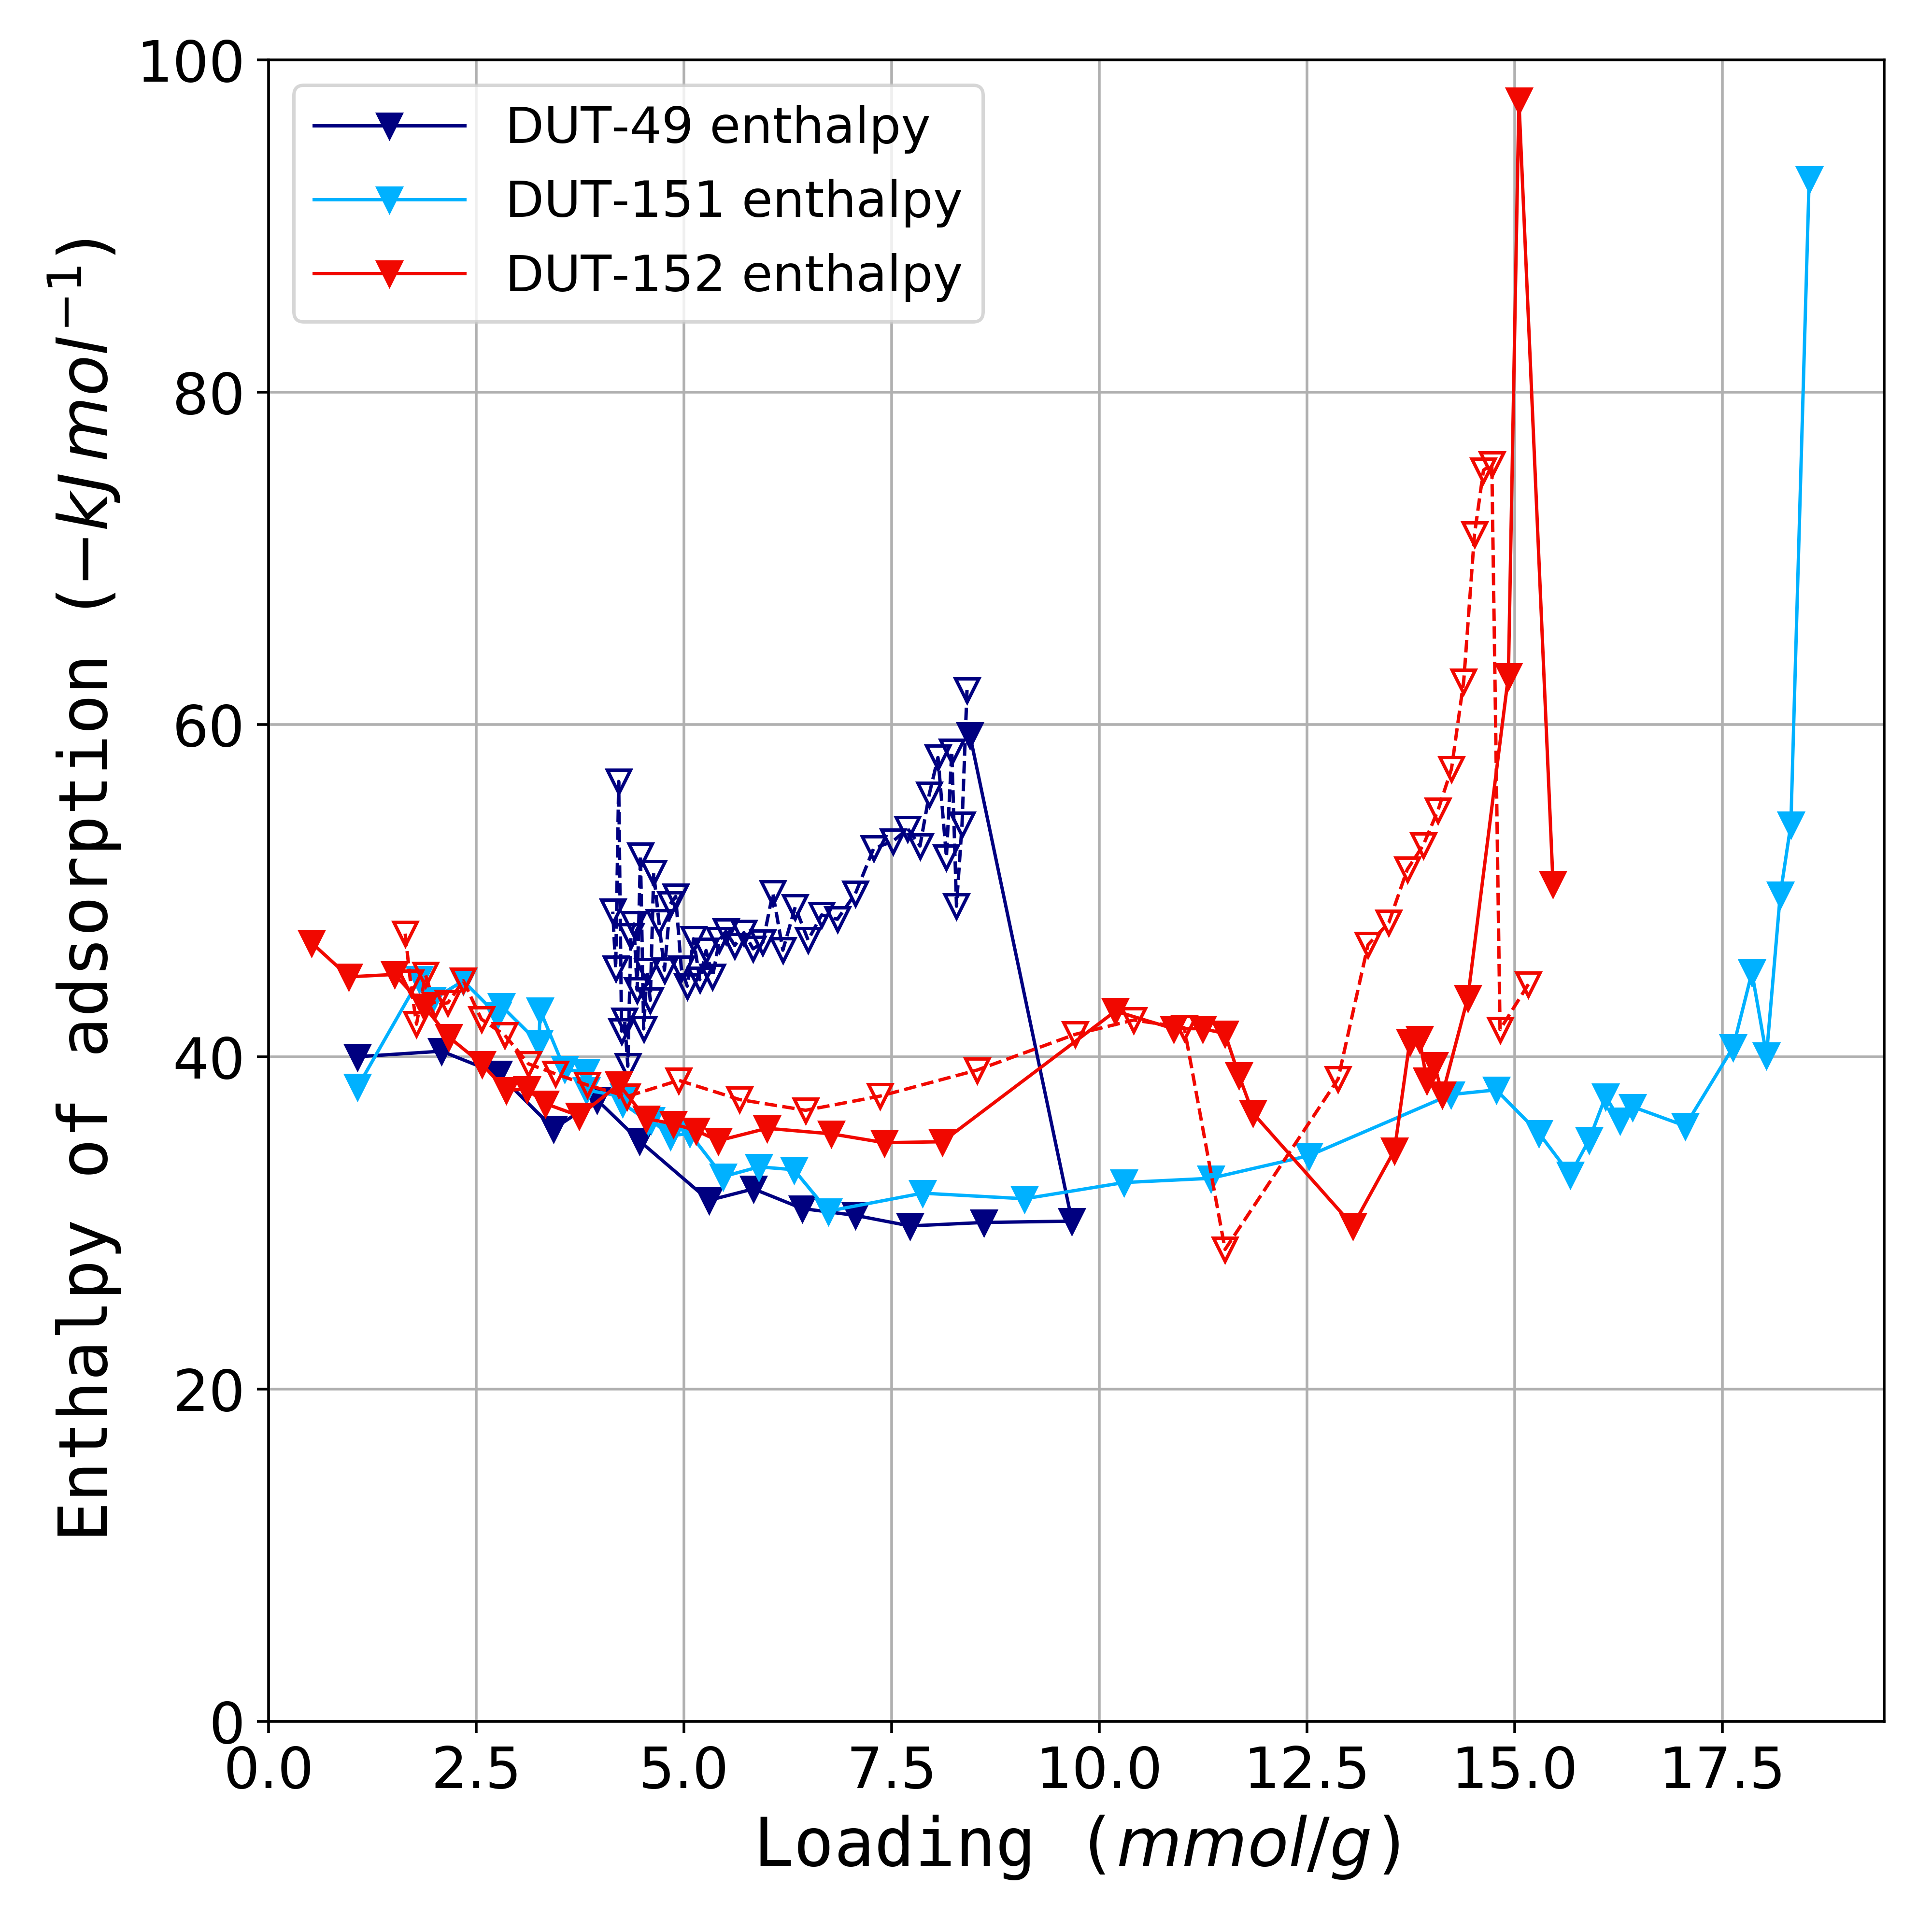
\includegraphics[width=\linewidth]{butane/dut-reticular-interp-enth}%
        \caption{}\label{dut:fgr:dut-reticular-interp-log}
    \end{subfigure}%
    \caption{The (a) isotherms and (b) enthalpy curves of the
    interpenetrated materials DUT-151 and DUT-152. Shaded regions
    are guides for the eye.}%
    \label{dut:fgr:dut-reticular-interp}
\end{figure}


\subsubsection{Behaviour of ``reinforced'' linker analogues}
